\documentclass[12pt]{article}

\usepackage[margin=1.0in]{geometry}
\usepackage{biblatex}
\addbibresource{citations.bib}
\usepackage{subfiles}
\usepackage{listings}
\lstset
{
	language=C,
	numbers=left,
	stepnumber=1,
	showstringspaces=false,
}
\usepackage{wrapfig}
\usepackage{setspace}
\doublespacing
\usepackage{pdfpages}
\usepackage{hyperref}

\urlstyle{same}

\begin{document}

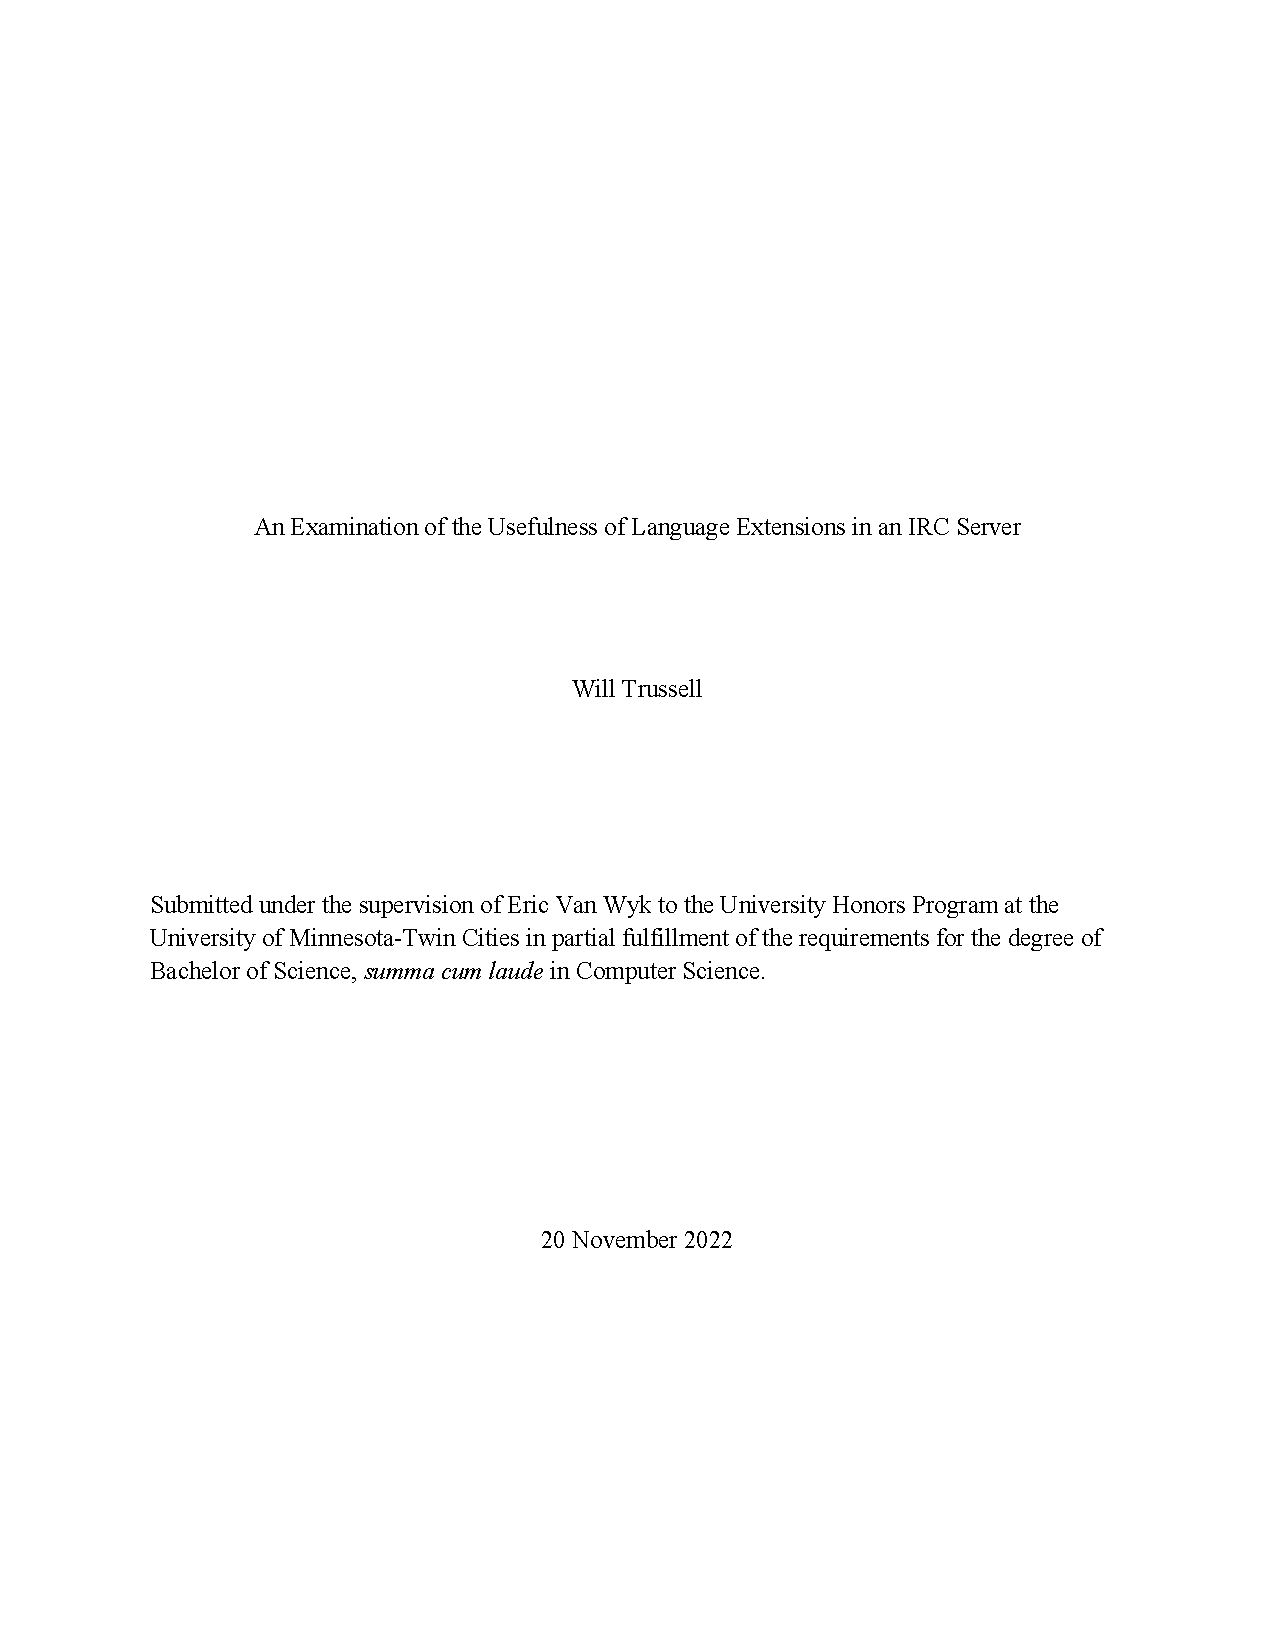
\includepdf[pages=-]{thesistitlepagetemplate_0.pdf}

\subfile{abstract.tex}

\newpage

\hypersetup{hidelinks}
\tableofcontents

\newpage

\subfile{Introduction.tex}
\newpage
\subfile{Background.tex}
\newpage
\subfile{nonnull.tex}
\newpage
\subfile{async.tex}
\newpage
\subfile{wuffs.tex}
\newpage
\subfile{discussion.tex}
\newpage
\subfile{future.tex}
\newpage
\begin{thebibliography}{99}
%%% TODO: Renumber all citations
	\bibitem{ngircd}
		A. Barton, “Next generation IRC daemon2,” ngIRCd, 2001. [Online]. Available: https://ngircd.barton.de/.
		[Accessed: 22-Nov-2022]. 


	%1
	\bibitem{aaron}
		Councilman, Aaron. (2021). An Extensible Implementation-Agnostic Parallel Programming Framework for C in ableC. Retrieved from the University of
		Minnesota Digital Conservancy, https://hdl.handle.net/11299/220246.

    %2
    \bibitem{silver}
        E. Van Wyk, D. Bodin, J. Gao, and L. Krishnan, “Silver: An extensible 
        attribute grammar system,” Electronic Notes in Theoretical Computer 
        Science, vol. 203, no. 2, pp. 103–116, Jan. 2010. 

	%3
    \bibitem{forwarding}
		E. Van Wyk, O. de Moor, K. Backhouse, and P. Kwiatkowski “Forwarding in 
        attribute grammars for modular language design,” Lecture Notes in 
        Computer Science, pp. 128–142, Apr. 2002.
    
    %4
    \bibitem{wuffs}
        Google, “Google/WUFFS: Wrangling untrusted file formats safely,” GitHub. 
        [Online]. Available: https://github.com/google/wuffs. [Accessed: 
        18-Nov-2022]. 
	
	%5
	\bibitem{McIlroy}
		M. D. McIlroy, “Macro instruction extensions of compiler languages,” 
        Communications of the ACM, vol. 3, no. 4, pp. 214–220, 1960. 
	
	%6
	\bibitem{IRC}
	    Oikarinen, J. and D. Reed, "Internet Relay Chat Protocol", RFC 1459, DOI 
        10.17487/RFC1459, May 1993, <https://www.rfc-editor.org/info/rfc1459>.
		
	%7
	\bibitem{ableC}
	    T. Kaminski, L. Kramer, T. Carlson, and E. Van Wyk, “Reliable and 
        automatic composition of language extensions to C: The ABLEC extensible 
        language framework,” Proceedings of the ACM on Programming Languages, 
        vol. 1, no. OOPSLA, pp. 1–29, 2017. 
\end{thebibliography}

\end{document}
